%!LW recipe=pdflatex-shellescape
\documentclass[11pt]{article}

\usepackage{geometry}
\geometry{margin=1in}

\usepackage[utf8]{inputenc}
%\usepackage[english]{babel}

\usepackage{graphicx}
\usepackage[dvipsnames]{xcolor}
\usepackage{amsmath}
\usepackage{float}
\usepackage{natbib}
\bibliographystyle{mnras}
\setcitestyle{authoryear,open={(},close={)}}
%\usepackage[hybrid]{markdown}
\usepackage{enumitem}
\setitemize{itemsep=-2pt}
\usepackage[colorlinks=true,allcolors=blue]{hyperref}
\usepackage{caption}
\usepackage{overpic}
\usepackage{amssymb}
\usepackage{multirow}
\usepackage{mathtools} 
\usepackage{lipsum}
\usepackage{fancyheadings}

\renewcommand{\subsectionmark}[1]{%
  \markright{\MakeUppercase{\thesubsection.\ #1}}}%

\pagestyle{fancy}
\fancyhead[L]{}
\fancyhead[R]{\nouppercase{\rightmark}}
\fancyfoot[R]{\vspace{-5pt}\rule{\textwidth}{0.4pt}\\ \thepage}
\fancyfoot[C]{\protect\color{gray}Compiled on \today}

\begin{document}

\tableofcontents
\clearpage

\section{Description of the system}

\subsection{Artificial chemistry}

Basically, we want to use a system based on artificial chemistry to investigate the conditions promoting the formation of complex objects---where, by "complex objects", we refer to molecular complexity. Specifically, we will be focusing our analysis on investigating the spatial topology of the environment, to try to determine how it can program the emergence of complexity. We will utilize Assembly Theory to quantify the complexity formed therein, and in doing so this model will constitute a new test environment. Among other things, this could help refine our methods of calculation for the Assembly Index, and inform our knowledge on how the Assembly Index responds to various parameters and/or is correlated to life-like properties.

Artificial chemistry implementations can be categorized along two axis: how abstract (or realistic) they represent "real" chemistry, and whether they aim to model early or late evolution (see~Fig.~\ref{fig:abstraction-stage}).

\begin{figure}[h]
  \centering
  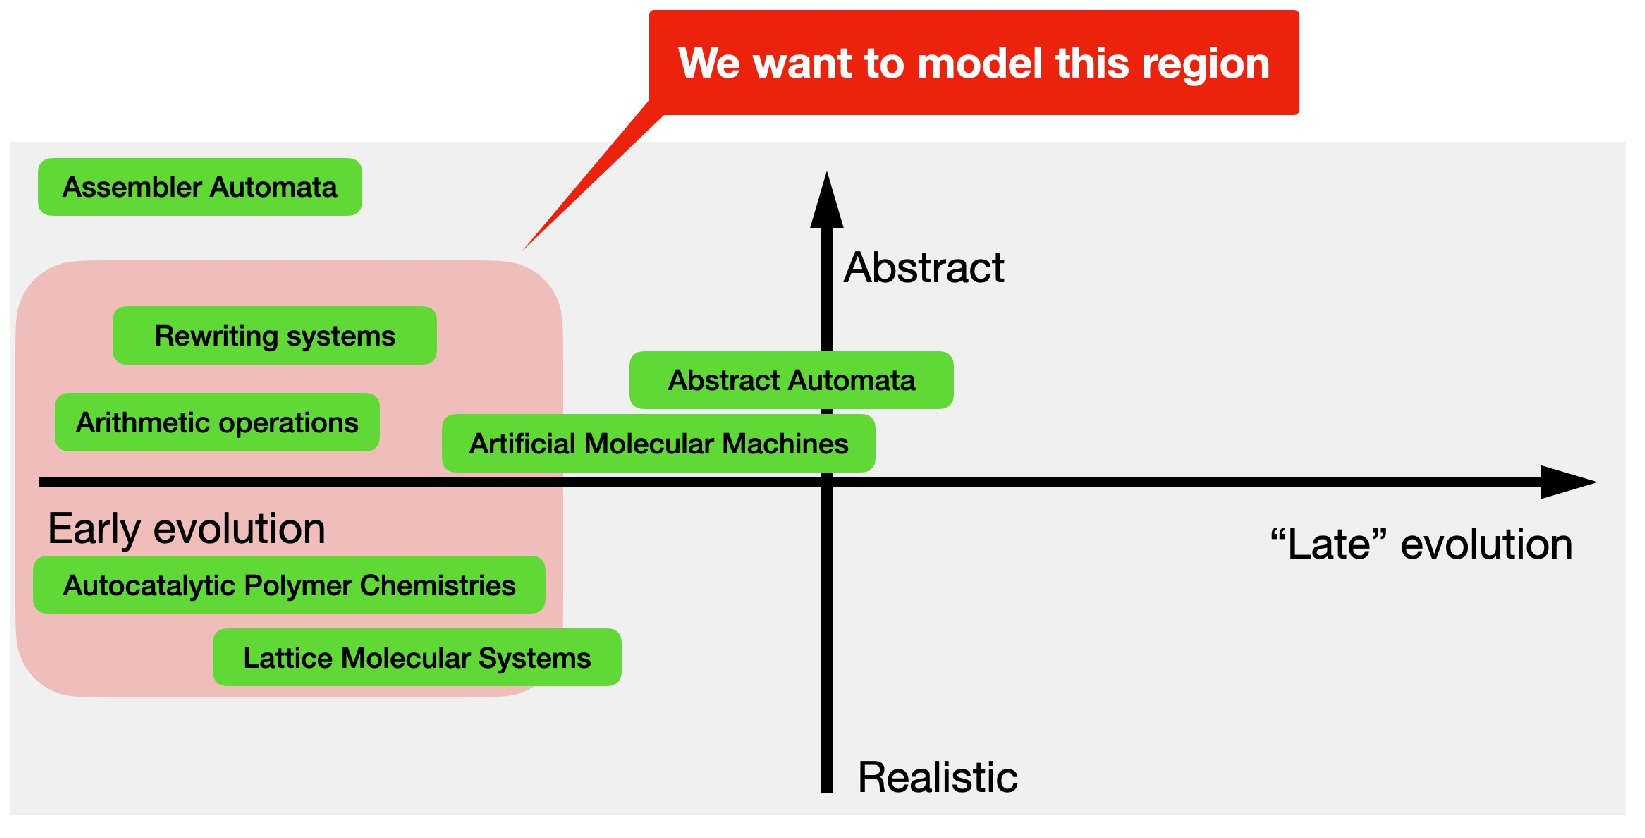
\includegraphics[width=0.75\textwidth]{figures/system/abstraction-stage.pdf}
  \caption{Classification of AC approaches along two axis: abstract vs realistic, and early vs late evolution. In the context of this project we will be focusing on the early evolution, using a balanced approach between more abstract and more realistic models.}
  \label{fig:abstraction-stage}
\end{figure}

The underlying (artificial) chemistry is based on several transformations: formard reactions, backward reactions, diffusion (Table~\ref{tab:reactions}. These reactions are parametrized by rate coefficients ($k_f$, $k_b$, $k_d$). Several other parameters can be defined, such as simulations (temporal) length $\tau_{max}$, the number of reactors $N$, the number of inflows $n$, total mass $M$, etc.

\begin{table}[h]
\centering
\begin{tabular}{|c|c|}
\hline Forward reaction & $A+B \xrightarrow{k_f} C$ \\
\hline Backward reaction & $C \xrightarrow{k_b} A^{\prime}+B$ \\
\hline \multirow{2}{*}{ Diffusion } & $C \xrightarrow{k_d} \varnothing$ \\
\cline { 2 - 2 } & $C_i \xleftrightarrow{k_d} C_j$ \\
\hline
\end{tabular}  
\caption{\color{red}\protect\lipsum[2]}
\label{tab:reactions}
\end{table}

\subsection{System of reactors}

These transformations are applied on a population of integers. These integers form a well-mixed system, inside a reactor/chemostat (Fig.~\ref{fig:reactor-ensemble}a). The number of integers \#1 is fixed, which translates into a fixed in-flow in the first reactor (as these integers are used to form other, more complex integers, or diffuse to the next chemostats). The system as a whole consists of several of these reactors, coupled together via in- and out-flows (defined by the corresponding rates), in a specific topology. For example, one of the simplest topology is that of the regular lattice (Fig.~\ref{fig:reactor-ensemble}b). When diffusion is very high, the whole system becomes well-mixed.

\begin{figure}[h]
  \centering
  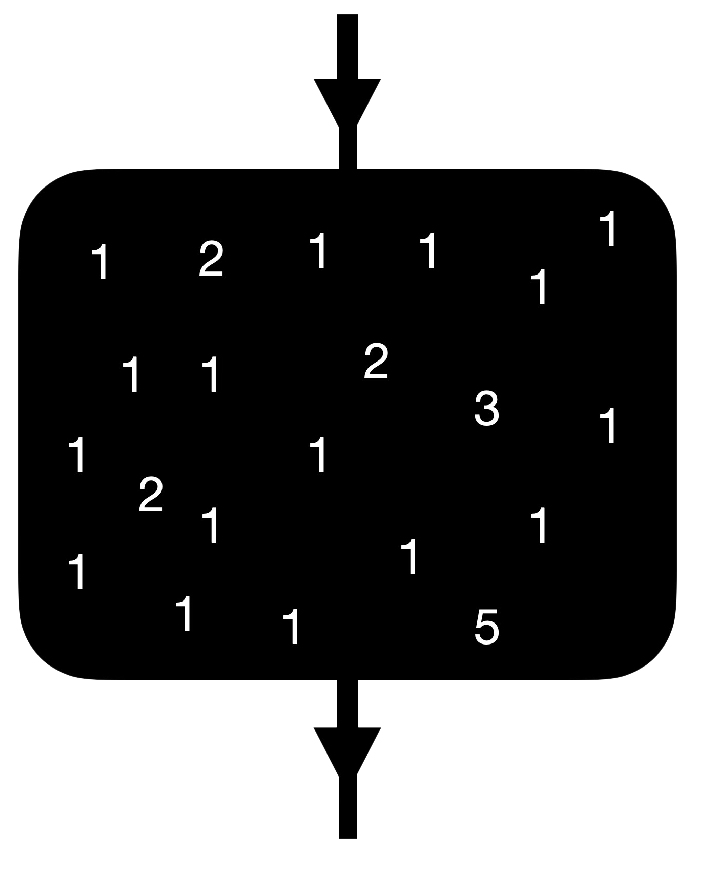
\includegraphics[width=0.25\textwidth]{figures/system/single-reactor.pdf}
  \hspace{0.10\textwidth}
  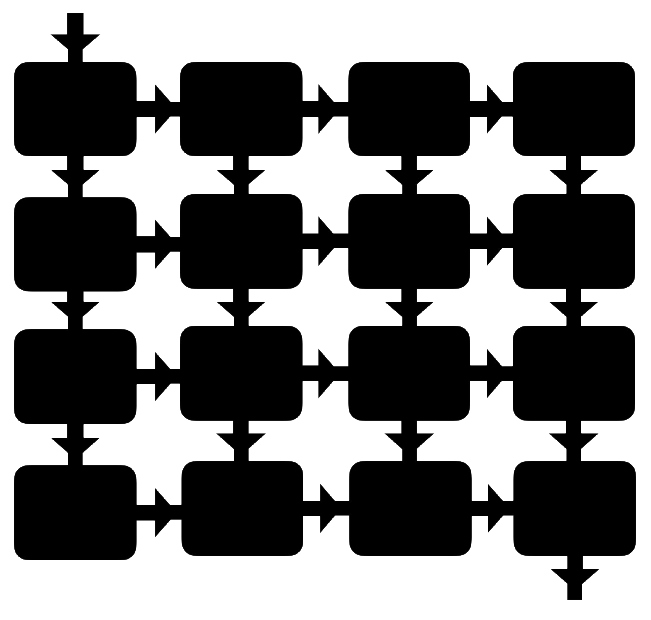
\includegraphics[width=0.30\textwidth]{figures/system/ensemble.pdf}
  \caption{\color{red}\protect\lipsum[2]}
  \label{fig:reactor-ensemble}
\end{figure}

\subsection{Topologies}

Several topologies can be used to connect the reactors together (Fig.~\ref{topologies}. Examples include: path, lattice, Erdos-Renyi (random), regular (uniform node degree) or Barabasi-Albert (power-law degree distribution). This is especially relevant given that we’re studying living systems, whose networks have been shown to possess certain specific properties deriving from their topology (e.g., resilience from BA networks, etc.) Other topologies (e.g. lattice, random) can be used as control/neutral.

\begin{figure}[h]
  \centering
  \begin{overpic}[width=0.05\textwidth]{figures/system/graph-path.pdf}\put(-15,95){\textbf{(A)}}\end{overpic}\hspace{1em}
  \begin{overpic}[width=0.20\textwidth]{figures/system/graph-lattice.pdf}\put(-15,100){\textbf{(B)}}\end{overpic}
  \begin{overpic}[width=0.20\textwidth]{figures/system/graph-ER.pdf}\put(-5,90){\textbf{(C)}}\end{overpic}
  \begin{overpic}[width=0.20\textwidth]{figures/system/graph-regular.pdf}\put(-15,90){\textbf{(D)}}\end{overpic}
  \begin{overpic}[width=0.20\textwidth]{figures/system/graph-BA.pdf}\put(-5,90){\textbf{(E)}}\end{overpic}
  \caption{\color{red}\\\textbf{Panel (A)} shows ...\\ \textbf{Panel (B)} shows ...\\ \textbf{Panel (C)} shows ...\\ \textbf{Panel (D)} shows ...\\ \textbf{Panel (E)} shows ...}
  \label{fig:topologies}
\end{figure}

\subsection{Integer chemistry and Assembly Theory}

{\color{red}\lipsum[2]}

\begin{figure}[h]
  \centering
  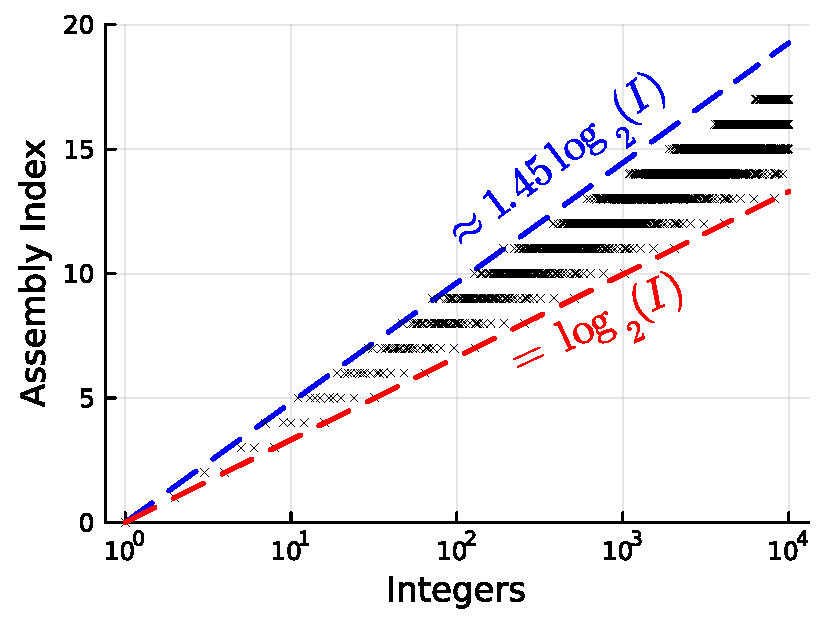
\includegraphics[width=0.40\textwidth]{figures/system/integers-assembly.pdf}
  \caption{\color{red}\protect\lipsum[2]}
  \label{fig:integers-assembly}
\end{figure}

\section{Experiments}

\subsection{Preliminary experiments (Sep-Oct 2024)}

{\color{red}\lipsum[2]}

\begin{figure}[h]
  \centering
  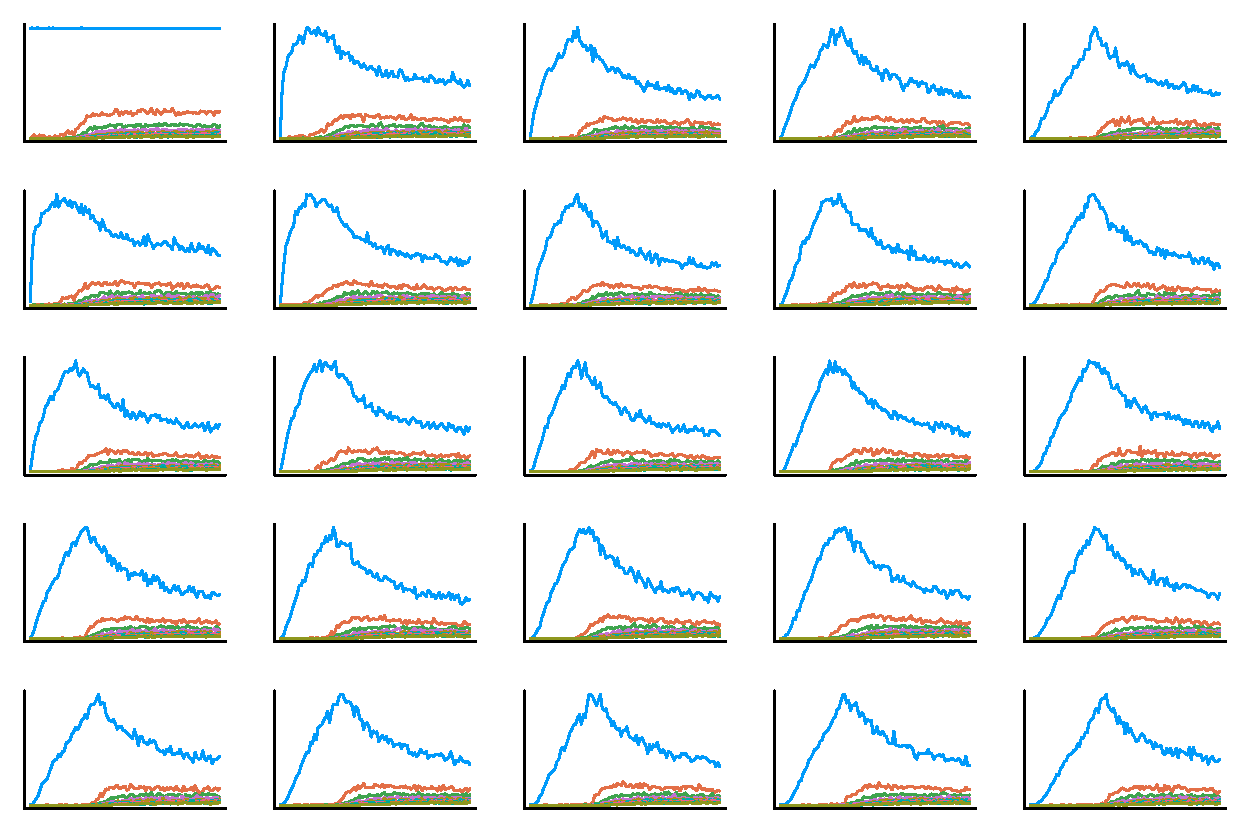
\includegraphics[width=0.55\textwidth]{figures/results/1-prelim/ts-gridplot.pdf}
  \caption{\color{red}\protect\lipsum[2]}
  \label{fig:}
\end{figure}

\subsubsection{Varying the diffusion rate}

Basically what we’ve done so far is vary the diffusion rate, plot the populations of chemical species across chemostats, and examine how the complexity varies when we change the diffusion. Here’s a few results (Fig.~\ref{fig:prelim})

\begin{figure}[h]
  \centering
  \begin{overpic}[width=0.30\textwidth]{figures/results/1-prelim/mu-vs-kd.pdf}\put(-5,80){\textbf{(A)}}\end{overpic}
  \begin{overpic}[width=0.30\textwidth]{figures/results/1-prelim/sd-vs-kd.pdf}\put(-5,80){\textbf{(B)}}\end{overpic}
  \begin{overpic}[width=0.30\textwidth]{figures/results/1-prelim/mass.pdf}\put(-5,80){\textbf{(C)}}\end{overpic} \\
  \caption{\color{red}\\\textbf{Panel (A)} shows ...\\ \textbf{Panel (B)} shows ...\\ \textbf{Panel (C)} shows ...}
  \label{fig:prelim-diffusion}
\end{figure}

\subsubsection{Measuring distance from source}

{\color{red}\lipsum[2]}

\begin{figure}[h]
  \centering
  \hspace{2em}
  \begin{overpic}[width=0.33\textwidth]{figures/results/1-prelim/ensemble-distance.pdf}\put(-15,80){\textbf{(A)}}\end{overpic}
  \hspace{0.10\textwidth}
  \begin{overpic}[width=0.40\textwidth]{figures/results/1-prelim/AI-vs-D.pdf}\put(-5,70){\textbf{(B)}}\end{overpic}
  \caption{\color{red}\\\textbf{Panel (A)} shows ...\\ \textbf{Panel (B)} shows ...}
  \label{fig:prelim-distance}
\end{figure}

\subsubsection{Measuring detection thresholds}

{\color{red}\lipsum[2]}

\begin{figure}[h]
  \centering
  \begin{overpic}[width=0.40\textwidth]{figures/results/1-prelim/abundance-I.pdf}\put(-5,70){\textbf{(A)}}\end{overpic}
  \hspace{0.05\textwidth}
  \begin{overpic}[width=0.40\textwidth]{figures/results/1-prelim/abundance-A.pdf}\put(-5,70){\textbf{(B)}}\end{overpic}
  \caption{\color{red}\\\textbf{Panel (A)} shows ...\\ \textbf{Panel (B)} shows ...}
  \label{fig:prelim-abundance}
\end{figure}

\subsubsection{Upcoming experiments}

\color{red}
\subsection{Title (date)}
\color{black}

{\color{red}\lipsum[2]}

\section{References}
%\bibliographystyle{apalike}
\footnotesize
\setlength{\bibsep}{0.0pt}
\bibliography{references-new.bib}

\end{document}
